%\documentclass[10pt,twocolumn,letterpaper,draft]{article}
\documentclass[10pt,letterpaper]{article}

% 使用中文宏包
\usepackage[UTF8]{ctex}
\usepackage{graphicx} %插入图片的宏包
\usepackage{float} %设置图片浮动位置的宏包
\usepackage{subfigure} %插入多图时用子图显示的宏包
%\usepackage[utf8]{inputenc}
\usepackage[strings]{underscore}
\usepackage{times}
\usepackage{epsfig}
\usepackage{amsmath}
\usepackage{amssymb}
\usepackage{overpic}
\usepackage{listings}
\usepackage{color}
\usepackage{enumitem}
\setenumerate[1]{itemsep=0pt,partopsep=0pt,parsep=\parskip,topsep=5pt}
\setitemize[1]{itemsep=0pt,partopsep=0pt,parsep=\parskip,topsep=5pt}
\setdescription{itemsep=0pt,partopsep=0pt,parsep=\parskip,topsep=5pt}

\definecolor{mygreen}{rgb}{0,0.6,0}
\definecolor{mygray}{rgb}{0.5,0.5,0.5}
\definecolor{mymauve}{rgb}{0.58,0,0.82}
\lstset{ %
  backgroundcolor=\color{white},   % choose the background color
  basicstyle=\footnotesize,        % size of fonts used for the code
  breaklines=true,                 % automatic line breaking only at whitespace
  captionpos=b,                    % sets the caption-position to bottom
  commentstyle=\color{mygreen},    % comment style
  escapeinside={\%*}{*)},          % if you want to add LaTeX within your code
  keywordstyle=\color{blue},       % keyword style
  stringstyle=\color{mymauve},     % string literal style
}

% Include other packages here, before hyperref.

% If you comment hyperref and then uncomment it, you should delete
% egpaper.aux before re-running latex.  (Or just hit 'q' on the first latex
% run, let it finish, and you should be clear).
\usepackage[pagebackref=true,breaklinks=true,letterpaper=true,colorlinks,bookmarks=false]{hyperref}


\def\httilde{\mbox{\tt\raisebox{-.5ex}{\symbol{126}}}}

\newcommand{\cmm}[1]{\textcolor[rgb]{0,0.6,0}{CMM: #1}}
\newcommand{\todo}[1]{{\textcolor{red}{\bf [#1]}}}
\newcommand{\alert}[1]{\textcolor[rgb]{.6,0,0}{#1}}

\newcommand{\IT}{IT\cite{98pami/Itti}}
\newcommand{\MZ}{MZ\cite{03ACMMM/Ma_Contrast-based}}
\newcommand{\GB}{GB\cite{conf/nips/HarelKP06}}
\newcommand{\SR}{SR\cite{07cvpr/hou_SpectralResidual}}
\newcommand{\FT}{FT\cite{09cvpr/Achanta_FTSaliency}}
\newcommand{\CA}{CA\cite{10cvpr/goferman_context}}
\newcommand{\LC}{LC\cite{06acmmm/ZhaiS_spatiotemporal}}
\newcommand{\AC}{AC\cite{08cvs/achanta_salient}}
\newcommand{\HC}{HC-maps }
\newcommand{\RC}{RC-maps }
\newcommand{\Lab}{$L^*a^*b^*$}
\newcommand{\mypara}[1]{\paragraph{#1.}}

\graphicspath{{figures/}}

\setcounter{page}{1}

\begin{document}
%\begin{CJK*}{GBK}{song}
 

%%%%%%%%% TITLE

\title{机器学习笔记}

\author{纳文琪$^{1}$}

\maketitle


\section{学习算法的性能度量\cite{2016机器学习}}
\subsection{错误率和精度}
\paragraph{错误率} 指的是分类错误的样本占总样本数的比例,主要适用于二分类问题,也可用于多分类问题。
\paragraph{精度} 指的是分类正确的样本数占总样本数的比例,同意适用于二分类和多分类问题。
\paragraph{} 错误率和精度简单、常用,但并不能满足所有需求。

\subsection{查准率、查全率和F1}
\paragraph{混淆矩阵} 对二分类问题,可以将真实类别与预测类别组合划分成TP、TN、FP、FN四种情形,分别表示预测正确的正例和反例、预测错误的
正例和反例。分类结果可以使用一个“混淆矩阵”表示:\\
\begin{figure}[H] %H为当前位置,!htb为忽略美学标准,htbp为浮动图形
	\centering %图片居中
	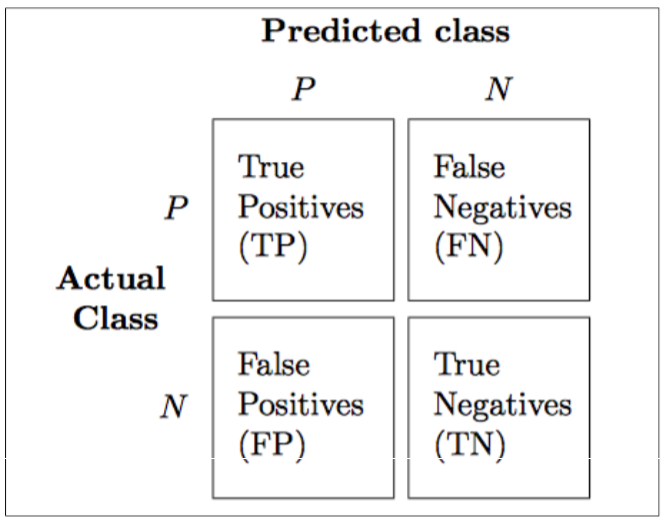
\includegraphics[width=0.7\textwidth]{../images/confusion_matrix.png} %插入图片,[]中设置图片大小,{}中是图片文件名
	\caption{Confusion Matrix} %最终文档中希望显示的图片标题
	\label{Fig.main2} %用于文内引用的标签
\end{figure}

\paragraph{查准率(准确率,precision)} 是从预测结果(其数量作为分母)出发计算的精度,指的是预测为正例的样本中,有多少的预测正确的。其定义是:\\
\begin{equation}
	P = \frac{TP}{TP + FP}
\end{equation}

\paragraph{查全率(召回率,recall)} 是从样本(其数量作为分母)出发计算的精度,指的是所有正例样本中,有多少被预测正确了。其定义是:\\
\begin{equation}
	R = \frac{TP}{TP + FN}
\end{equation}

\paragraph{} 查全率与查准率是一对矛盾的度量。

\paragraph{P-R曲线} 用于直观地显示学习器在样本总体上的查全率、查准率。

\paragraph{F1和$F_\beta$} F1是综合考虑查全率和查准率的度量,定义为:\\
\begin{equation}
	F1 = \frac{ 2 \times P \times R }{P + R}
\end{equation}
一些应用中,对查准率和查全率的重视程度不同,此时需要用$F_\beta$ : \\
\begin{equation}
	F_\beta = \frac{ (1+\beta^2) \times P \times R }{(\beta^2 \times P) + R}
\end{equation}
$F_\beta$是F1的一般形式,当$\beta = 1$时就是F1;当$\beta > 1$时,查全率有更大影响;当$\beta < 1$时,查全率有更大影响。

\subsection{ROC与AUC}
\paragraph{ROC} 全称是“受试者工作特征”,与P-R曲线类似,它也有两个坐标,其纵坐标表示的是“真正例率”(TPR),即正例的查全率,横坐标表示的是“假正例率”,及反例被判断错误的比率。两者定义为:\\
\begin{equation}
	TPR = \frac{TP}{TP + FN}
\end{equation}
\begin{equation}
	FPR = \frac{FP}{TN + FP}
\end{equation}
ROC曲线的对角线对应的是“随机猜想”模型,而点(0,1)则代表“理想模型”。

\paragraph{AUC} 进行学习器比较时,与P-R曲线类似,若一个学习器的ROC曲线被另一个学习器的曲线完全包住,则可断言后者的性能优于前者;若两个学习器的ROC曲线有交叉,则需要比较ROC曲线下的面积,即AUC来进行判断。
\newpage
\section{线性模型}
\subsection{LMNN}
\paragraph{} kNN成功的关键是对距离度量方法的选择,一般我们都会选欧氏距离作为距离度量方法,但这并不一定都会有效。理想情况下,我们应该根据具体的问题来选择距离度量方法,基于特定样本,学习一个特定的距离度量方法可以使得kNN的性能得到改善。
\paragraph{} LMNN就是通过样本学习一个线性变换M,而样本之间的距离则通过M进行度量。如下图:
\begin{figure}[H] %H为当前位置,!htb为忽略美学标准,htbp为浮动图形
	\centering %图片居中
	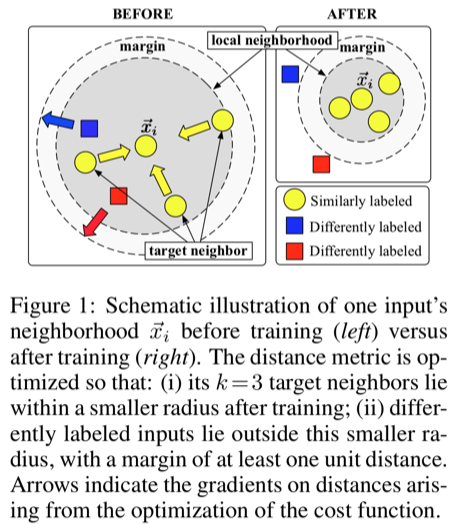
\includegraphics[width=0.7\textwidth]{../images/lmnn.png} %插入图片,[]中设置图片大小,{}中是图片文件名
	\caption{Confusion Matrix} %最终文档中希望显示的图片标题
	\label{Fig.main2} %用于文内引用的标签
\end{figure}
之前是默认的欧式距离的度量,正样本与负样本之间的距离差不多,之后是通过学习得到的新的度量方法所获得的效果。

\newpage
\section{神经网络}

\paragraph{隐层参数} $W_j \in \mathbb{R}^{d  \times n}$ 表示j-th层的参数,此层有n个神经元,接收d个来自的(j-1)-th层的输入。$W_j$的第k列,就是输入到第k个神经元的数据对应的参数。
\paragraph{隐层输出} $y_j \in \mathbb{R}^n$ 表示j-th层的输出,n个神经元有n个输出,计算公式为:$y_j = W_j^Ty_{j-1}+b_j$

\newpage
\section{Deep Neural Networks for Bot Detection\cite{kudugunta2018bot}}

\paragraph{Motivation} 现有的系统都是在account-level进行bots的发现,需要根据特定帐号的一系列历史活动记录来确认帐号是否是bot。这在进行检测的时候代价非常昂贵。论文希望通过仅仅一条tweet来判断是否是bot。

\paragraph{} 论文将bot发现的方法分为用户级和tweet级,进行分类;tweet级根据
\paragraph{数据集} 论文使用的数据集存在不平衡问题,作者分别使用SMOTE+ENN和SOMTE+TOMEK的方法平衡数据。数据分为用户级和tweet级两类,用户级数据(用户元数据)包括statuses count、followers count等,tweet级数据包括retweet count、number of hashtags等。

\newpage
\section{损失函数}
\subsection{softmax}
\paragraph{下溢(underflow)} 当接近零的数被四舍五入为零后发生下溢。
\paragraph{上溢(overflow)} 当大数量级的数被近似为$\infty$或$-\infty$时,发生上溢。 
\paragraph{softmax函数}可对下溢和上溢进行数值稳定,定义为:
\begin{equation}
	softmax(\mathbf{x})_i = \frac{exp(x_i)}{\sum^n_{j=1}exp(x_j)}
\end{equation}
这个式子同样会产生溢出,例如,当x是很小的负数时,分母会变成零;当x是很大的数时,一样会发送上溢。这个问题可以通过计算$softmax(\mathbf(z), z=x-\max_ix_i$ 同时解决。

\newpage
\section{A Discriminative Feature Learning Approach for Deep Face Recognition \cite{centerloss}}
\subsection{Introduction}
\paragraph{动机} 一般的物体识别,主要是闭集识别,利用softmax loss即可处理,但人脸识别不单需要特征可分离(separable),也需要可区分(discriminative),构建一个高效的loss可提升可区别性,为此,本文提出center loss。

\paragraph{Center loss} 为每一个class的特征维护一个center,每次进行SGD的时候同时更新center,并最小化class中样本特征到中心的距离。
\subsection{The Proposed Approach}
\paragraph{toy example} 本文使用一个toy example来演示算法的效果。它最后一个隐层的维度是2,以便于我们使用二维图像来显示特征分布。toy example使用softmax loss,最后输出的特征的分布表示为图\ref{softmax-loss-2-d} :
\begin{figure}[H]
	\centering
	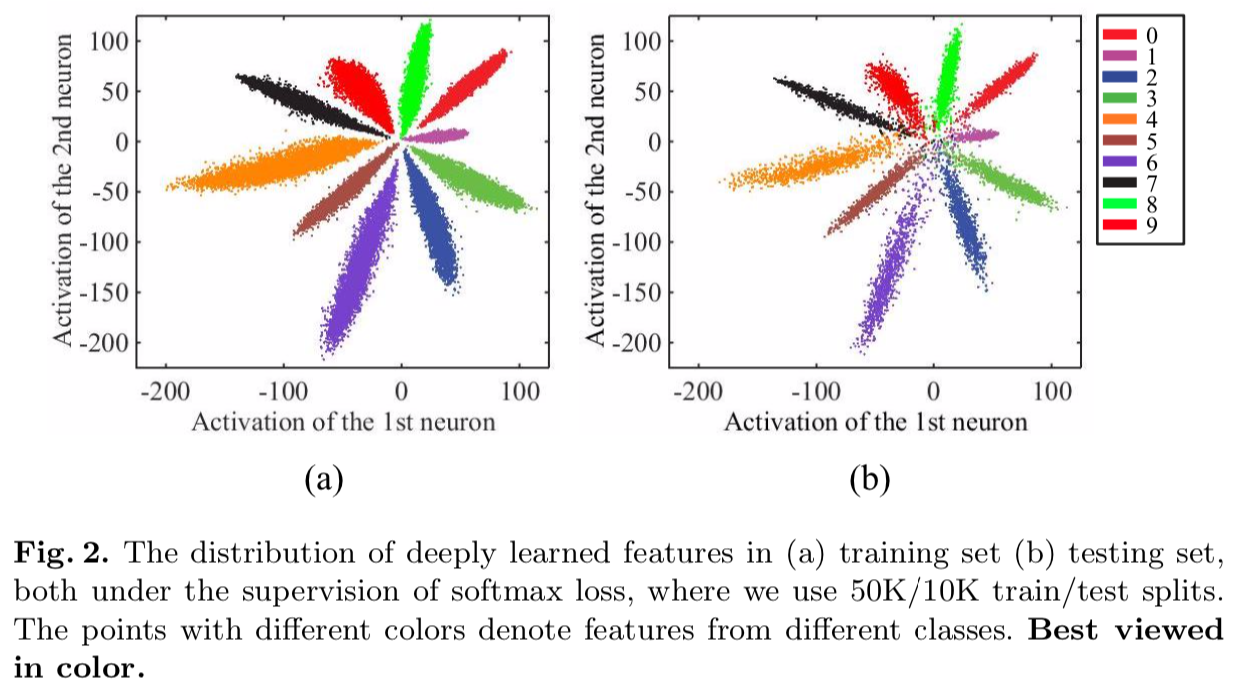
\includegraphics[width=0.9\textwidth]{../images/softmax-loss-2-d.png}
	\caption{}
	\label{softmax-loss-2-d}
\end{figure}

\paragraph{Center loss} 为增强可区分度,需在保持特征分类的同时,最小化内部class的方差。center loss定义为:
\begin{equation}
	\mathfrak{L}_C=\frac{1}{2}\sum^m_{i=1}\left \| \mathbf{x}_i-\mathbf{c}_{y_i} \right \|^2_2
\end{equation}
理论上,$c_{y_j}$应当随着特征的变化而更新,因此,在每次更新更新参数的时候都要对它进行更新。
\paragraph{} 综上,总的损失函数可以表示为:
\begin{equation}
	\mathfrak{L} = \mathfrak{L}_S + \lambda \mathfrak{L}_C
\end{equation}
\begin{figure}[H]
	\centering
	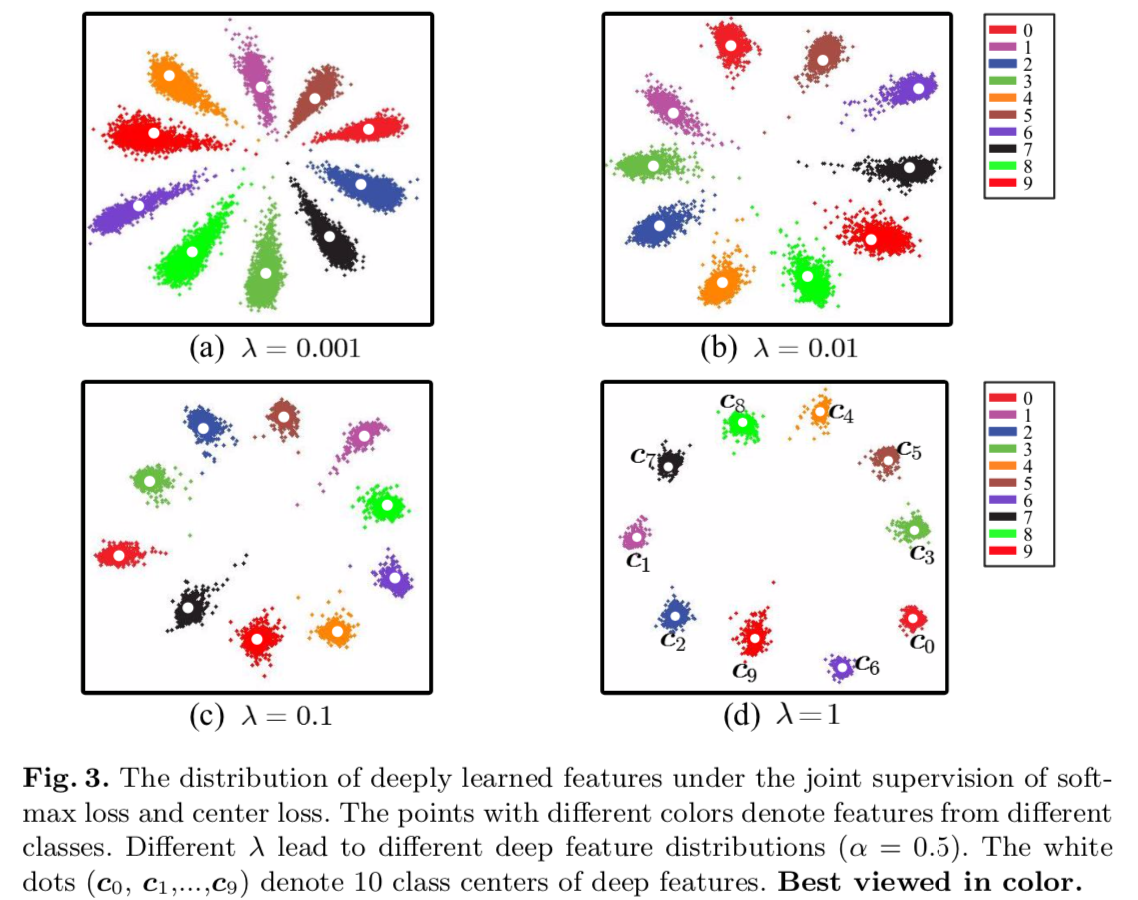
\includegraphics[width=0.9\textwidth]{../images/center-loss.png}
	\caption{}
	\label{softmax-loss-2-d}
\end{figure}


\newpage
\section{Large-Margin Softmax Loss for Convolutional Neural Networks\cite{l-softmax}}
\paragraph{} 为通过可区分的信息来增强CNN性能,本文提出一种新的损失函数L-Softmax。它通过用特征化的方法来将样本与参数划分开。如图所示,第一列是普通的softmax,后面的是l-softmax,使用l-softmax会使学习到的特征更加紧凑和区分良好(well separated):
\begin{figure}[H]
	\centering
	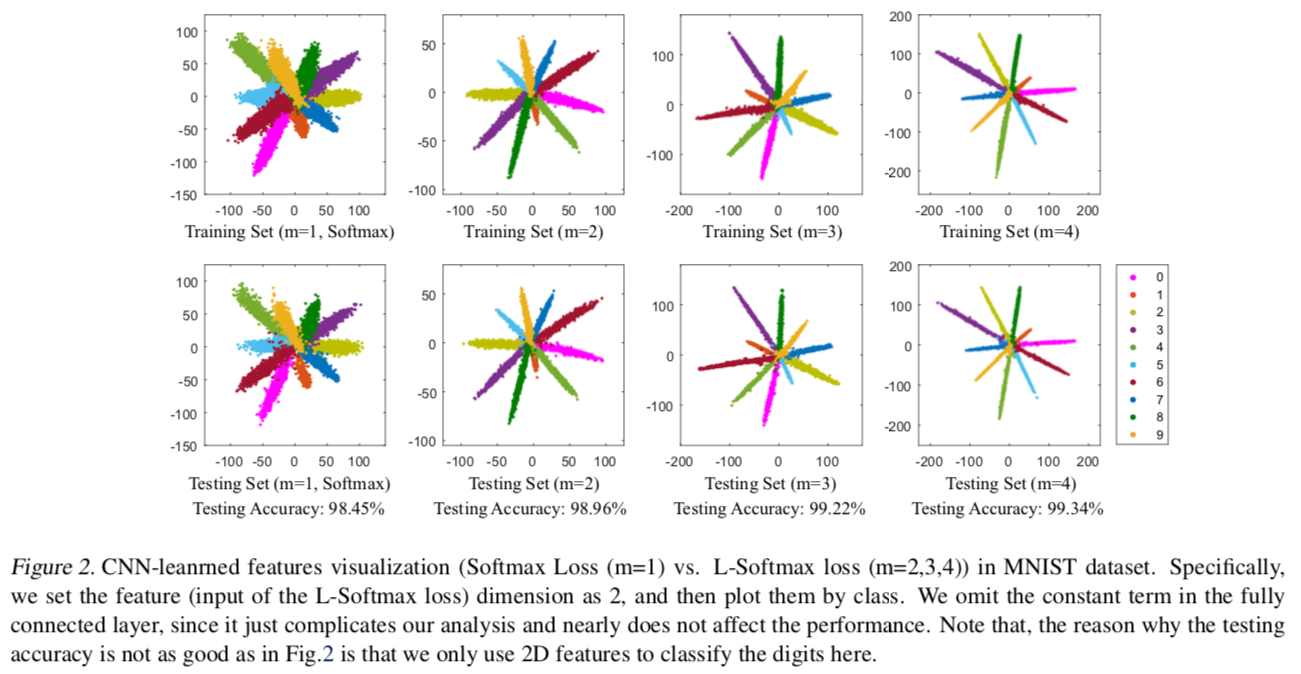
\includegraphics[width=1\textwidth]{../images/l-softmax.png}
	\caption{}
	\label{l-softmax}
\end{figure}

\subsection{基础}
\paragraph{} 由于矩阵的积可以表示为:$W_j^Tx_i = \left \| W_j \right \|\left \| x_i \right \|\cos(\theta_j)$,因此,softmax可以表示为:
\begin{equation}
	softmax(\mathbf{x})_i = \frac{\exp(\left \| W_{y_i} \right \|\left \| x_i \right \|\cos(\theta_{y_i}))}{\sum^n_{j=1}\exp(\left \| W_j \right \|\left \| x_i \right \|\cos(\theta_j))}
\end{equation}
\paragraph{} 假设一个2分类问题,如果x输入分类1,则softmax肯定会希望属于分类1的概率比分类2大,也就是$W_1^Tx > W_2^Tx$,用上面的式子替换就是:$\left \| W_1 \right \|\left \| x \right \|\cos(\theta_1) > \left \| W_2 \right \|\left \| x \right \|\cos(\theta_2)$。然而,我们为了获得更加严格的分类边界,可以要求:$\left \| W_1 \right \|\left \| x \right \|\cos(m\theta_1) > \left \| W_2 \right \|\left \| x \right \|\cos(\theta_2) (0 \leq \theta_1 \leq \frac{\pi}{m} )$,这里m是一个正整数。

\subsection{定义}
\paragraph{} 根据以上信息,我们可以定义L-softmax为:
\begin{equation}
	L_i = -\log(\frac{\exp(\left \| W_{y_i} \right \|\left \| x_i \right \|\cos(\theta_{y_i}))}{\exp(\left \| W_{y_i} \right \|\left \| x_i \right \|\psi(\theta_{y_i})) + \sum_{j\neq y_i }\exp(\left \| W_j \right \|\left \| x_i \right \|\cos(\theta_j))} )	
\end{equation}
上式中,$\psi(\theta)$ 应该是一个单调递减函数,而$\cos(m\theta)$函数仅在$0 \leq \theta_1 \leq \frac{\pi}{m} $范围内是单调递减的。因此,这里需要引入一个新的单调递减函数$D(\theta)$,并且$D(\frac{\pi}{m})=\cos(\frac{\pi}{m})$。这样的话,$\psi(\theta)$就可以定义为:
\begin{equation}
	\psi(\theta) = \left \{ \begin{matrix}
		\cos(m\theta), 0 \leq \theta \leq \frac{\pi}{m}
		\\ 
		D(\theta), \frac{\pi}{m} \leq \theta \leq \pi
	\end{matrix}\right.
\end{equation}
\subsection{几何解释}
\paragraph{}从以下图中可以直观看出决策边界的变化:
\begin{figure}[H]
	\centering
	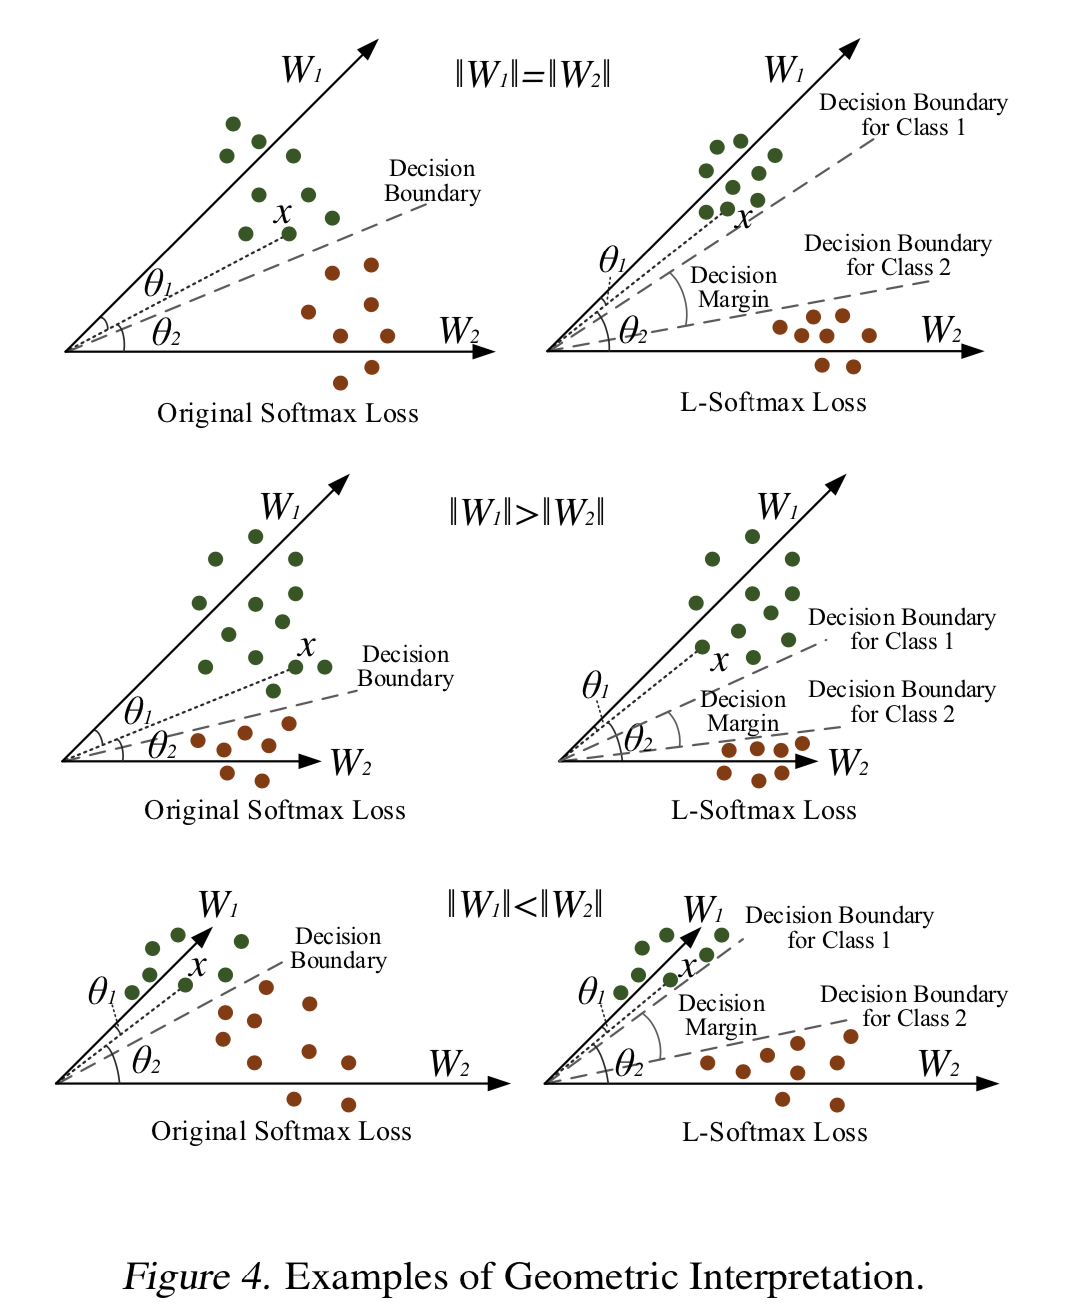
\includegraphics[width=0.6\textwidth]{../images/l-loss-geo.png}
	\caption{}
	\label{l-softmax 集合解释}
\end{figure}


\newpage
\section{FaceNet: A Unified Embedding for Face Recognition and Clustering\cite{facenet}}
\paragraph{} 本文提出一种可同时用于人脸验证(是否是同一个人)、识别(这是谁)和聚类(找出相同的脸)的系统,其主要基于CNN为每个图像学习一个欧几里得嵌入,越相似的脸,他们之间的距离就越小。一旦学习到嵌入,验证问题就是比较两个嵌入的距离,识别问题就是一个kNN分类问题,聚类就是普通聚类问题。
\paragraph{FaceNet} 基于LMNN方法,使用一个三元组(triplet)将图像训练输出为一个128维的嵌入。triplet由两个匹配的人脸图片和一个不匹配的人脸图片组成,损失函数的目的是让一个样本与他的正样本尽可能靠近,与他的负样本尽可能分离。

\paragraph{模型结构} 把CNN看成一个黑盒子,模型可以表示为:
\begin{figure}[H]
	\centering
	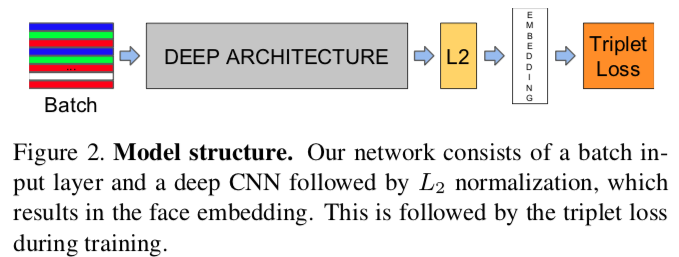
\includegraphics[width=0.9\textwidth]{../images/facenet-model.png}
	\caption{}
	\label{FaceNet Model}
\end{figure}
该模型使用的损失函数是triplet loss,最终目的是训练一个从图像$x$到特征空间$\mathbb{R}^d$的嵌入$f(x)$,使得相同的脸之间的距离较小,不同脸之间的距离较大。
\paragraph{Triplet loss} 上述嵌入表示为$f(x) \in \mathbb{R}^d$,且限制在一个单位超球体内,即要求$\left \|f(x) \right \|_2=1$。通过这个损失函数,我们希望确保一个人的图像$x_i^a$(anchor)与其他同是这个人的图像$x_i^p$(positive)距离更加,与其他人的图像$x_i^n$(negative)距离更远。如图所示:
\begin{figure}[H]
	\centering
	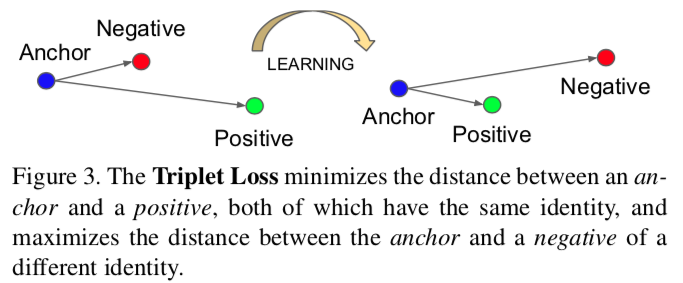
\includegraphics[width=0.9\textwidth]{../images/triplet-loss.png}
	\caption{}
	\label{Triplet Loss}
\end{figure}
可以表示为:
\begin{equation}
	\left \| x_i^a - x_i^p \right \|_2^2 + \alpha < \left \| x_i^a - x_i^n \right \|_2^2, \forall(x_i^a, x_i^p, x_i^n) \in \tau
\end{equation}
其中,$\alpha$是一个边界值。总体的损失函数即可定义为最小化:
\begin{equation}
	L=\sum_i^N \left [ \left \| f(x_i^a) - f(x_i^p) \right \|_2^2 - \left \| f(x_i^a) - f(x_i^n) \right \|_2^2 + \alpha \right ]_+
\end{equation}
学习的过程就是生成三元组,然后最小化L。
\paragraph{Triplet的选择} 如果生成全部可能的三元组用于学习,将会导致有很多三元组很容易满足公式(13),这些无用的三元组会导致收敛速度变慢,因此,我们需要选择那些违反了公式(13)的三元组来进行训练。也就是说,给定$x_i^a$,我们应该选择距离它最远的$x_i^p$(hard positive)(argmax),以及距离它最近的$x_i^n$(hard negitive)(argmin)。然而,这种方式并不容易处理,因为会有一些标记错误的样本严重影响训练过程。我们有两种方法避免这个问题:
	\subparagraph{离线生成} 每隔n次训练之后,使用最近的网络参数计算argmax和argmin;
	\subparagraph{在线生成} 在mini-batch中选择。
	
\paragraph{在线选择三元组} 为了获得有意义的距离表示,在每一个mini-batch中必须保证有一定数量的positive样本。本文在数千个样本的mini-batch中要求40个左右的positive样本。选择positive是,我们选最远的那个,而选择negitive时,我们选所有的negitive样本。



\newpage
\bibliographystyle{ieeepes}
\bibliography{../Saliency}
\end{document}



























































